\section{Vakkarima vastagsága és karima szabványok}

\begin{figure}[hbt!]
	\centering
	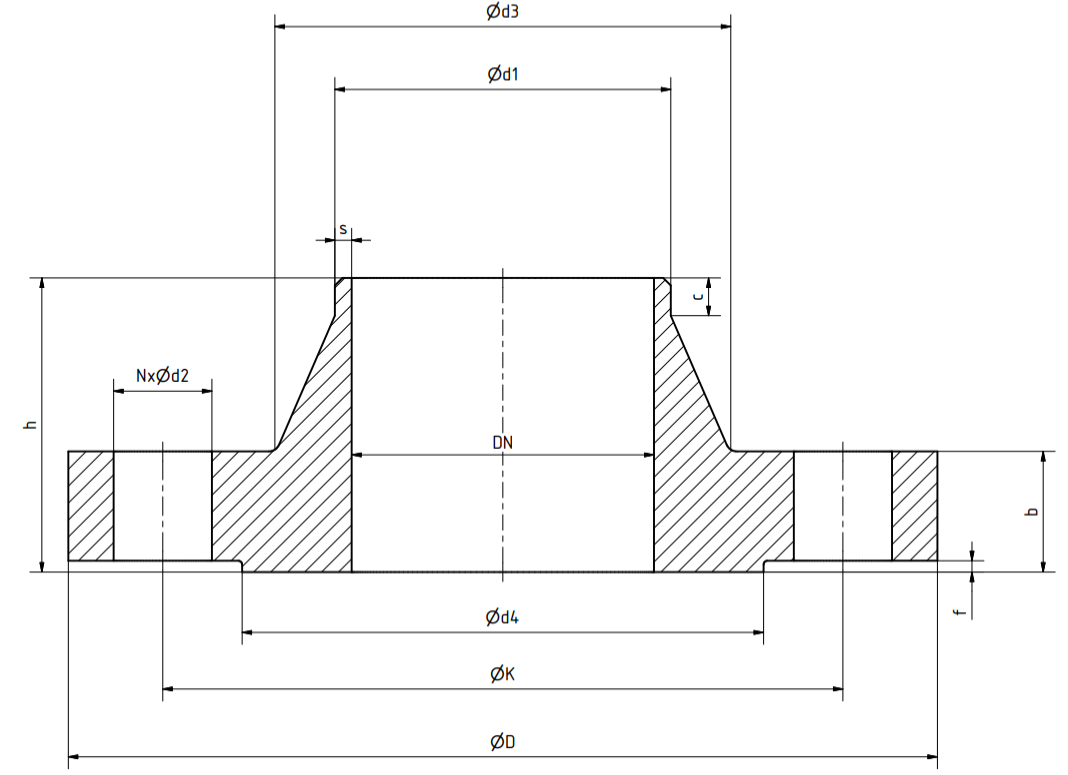
\includegraphics[scale=.61]{./images/karima.png}
	\caption{Karima előtervének rajza}
\end{figure}
\begin{align*}
	&D = \siunit{\karimaD}{\mm} \\
	&f = \siunit{\karimaf}{\mm} \\
	&d_4 = \siunit{\karimadfour}{\mm} \\
	&d_2 = \siunit{\karimadtwo}{\mm} \\
	&s = \siunit{\karimas}{\mm} \\
	&N = \siunit{\karimaN}{db} \\
	&K = \siunit{\karimaK}{\mm} \\
	&b = \siunit{\karimab}{\mm} \\
	&d_3 = \siunit{\karimadthree}{\mm} \\
	&d_1 = \siunit{\karimadone}{\mm} \\
	&M = \text{M24} \\
	&h = \siunit{\karimah}{\mm} \\
\end{align*}

\newpage
\begin{figure}[hbt!]
	\centering
	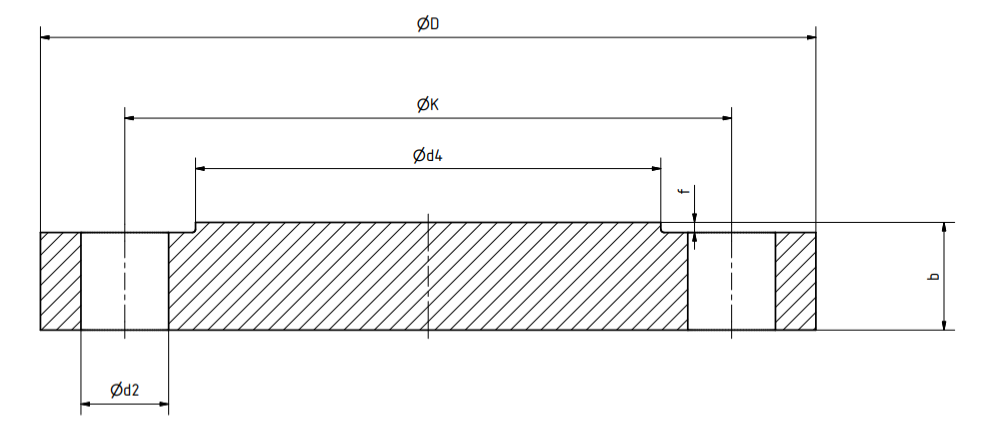
\includegraphics[scale=.34]{./images/vakkarima.png}
	\caption{Vakkarima előtervének rajza}
\end{figure}
\begin{align*}
	&D = \siunit{\karimaD}{\mm} \\
	&f = \siunit{\karimaf}{\mm} \\
	&d_4 = \siunit{\karimadfour}{\mm} \\
	&d_2 = \siunit{\karimadtwo}{\mm} \\
	&K = \siunit{\karimaK}{\mm} \\
	&b = \siunit{\karimab}{\mm} \\
\end{align*}
